\begin{figure}[h]
    \centering
    \begin{subfigure}[b]{0.56\textwidth}
        \centering
        \caption{}
        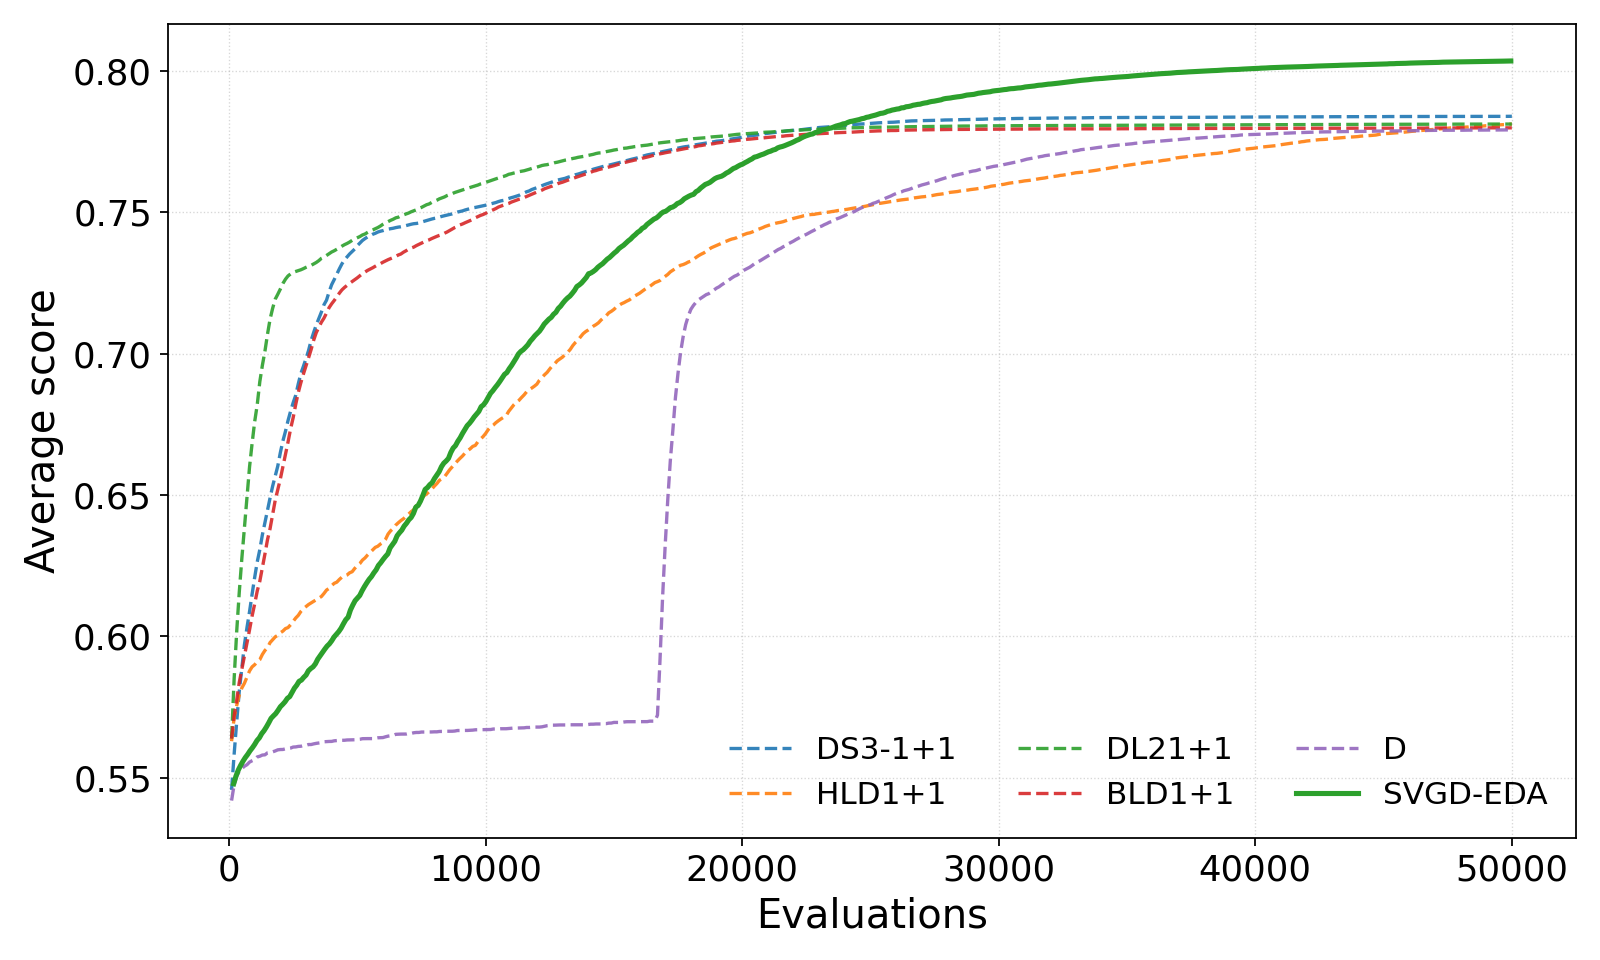
\includegraphics[width=\linewidth]{comparison_nk3_256_t2.png}
        \label{fig:comparison_nk3_256_t2}
    \end{subfigure}
    \vspace{0.5cm}
    \begin{subfigure}[b]{0.42\textwidth}
        \centering
        \caption{}
        
\includegraphics[width=\linewidth]{boxplot_final_score_vs_top5.png}
        \label{fig:boxplot_nk3_256_t2}
    \end{subfigure}

    \caption{Performance analysis on a NK3 instance distribution ($n=256, K=2$). (a) Evolution of the average score for \texttt{SVGD-EDA} and the top-five competitors. (b) Final score distribution after 50,000 evaluations. Both panels use the same labels/colors: SVGD-EDA, DS3-1+1, HLD1+1, DL21+1, BLD1+1, D. Acronyms in legends: DS3-1+1 = \texttt{DiscreteLengler3OnePlusOne}; HLD1+1 = \texttt{HugeLognormalDiscreteOnePlusOne}; DL21+1 = \texttt{DiscreteLengler2OnePlusOne}; BLD1+1 = \texttt{BigLognormalDiscreteOnePlusOne}; D = \texttt{discretememetic}.}
    \label{fig:benchmark_plots_nk3_256_t2}
\end{figure}
